\section{Specifications}
\label{sec:specs}
\newcounter{SpecID}

\subsection{Arena}
\refstepcounter{SpecID}
\label{spec:arena}

\begin{enumerate}
  \item The arena floor is a \SI{6}{m} $\times$ \SI{12}{m} rectangle.
  \item The layout of the arena is given in Figure~\ref{fig:arena}. This
        figure is to scale.
  \item The docking area is \SI{1.5}{m} $\times$ \SI{1.5}{m}.
  \item The raised areas are each \SI{1.5}{m} $\times$ \SI{1}{m}, and raised
        from the floor by \SI{0.5}{m}.
  \item The starting zones are centrally aligned, share one side with the
        north wall of the arena, and are \SI{0.9}{m} $\times$ \SI{0.9}{m}.
  \item The canonical definition of the arena is what is in the simulator.
\end{enumerate}

\begin{figure}
  \centering
  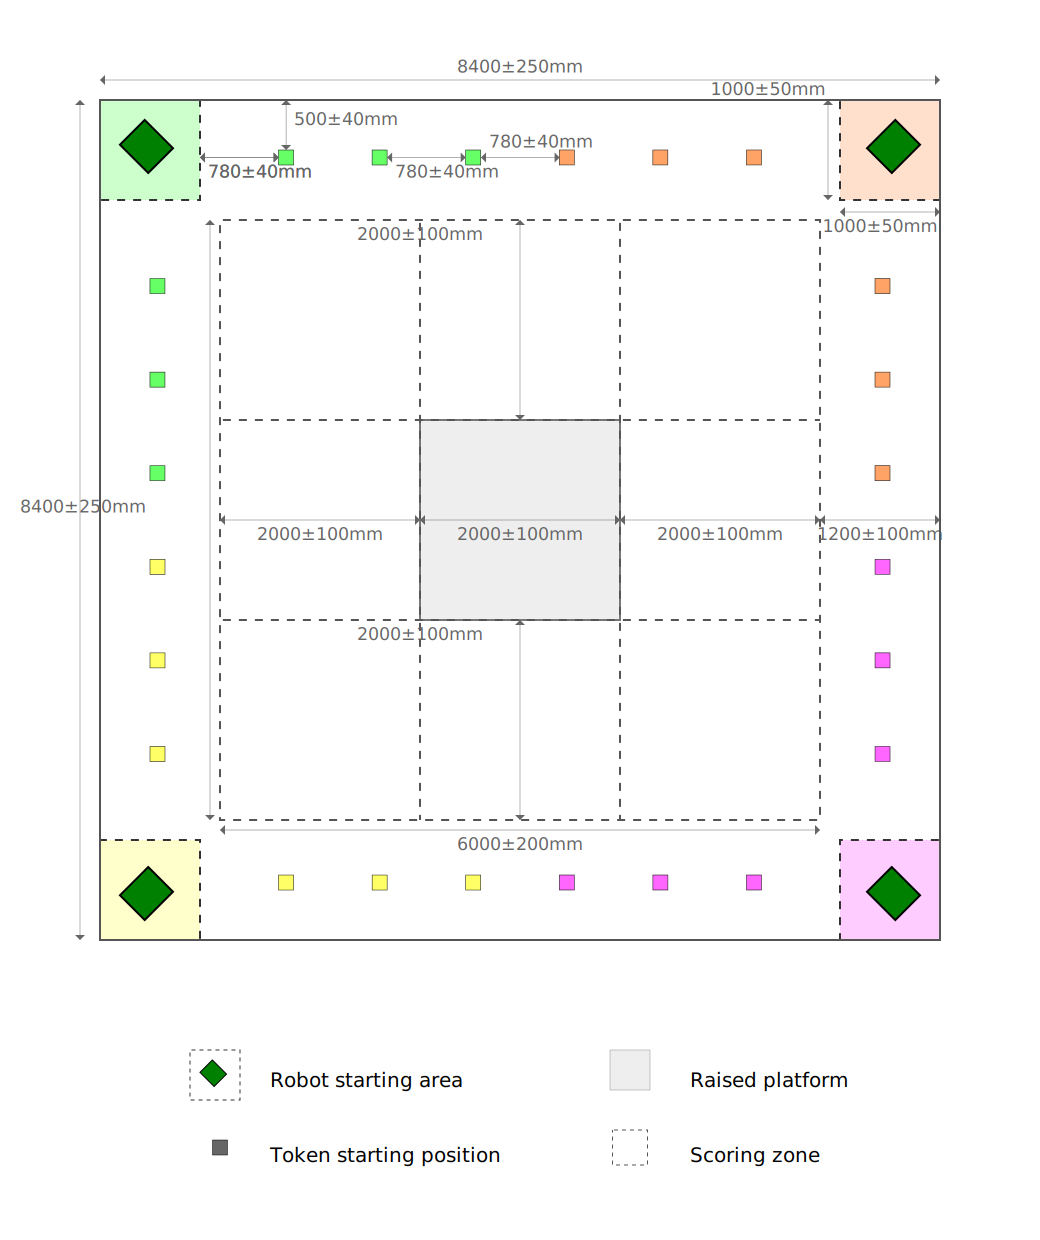
\includegraphics[scale=0.58]{fig-arena.pdf}
  \caption{Layout zones and tokens in the arena.}
  \label{fig:arena}
\end{figure}

\subsection{Containers}
\refstepcounter{SpecID}
\label{spec:containers}

\begin{enumerate}
  \item Containers are cuboids with side length \SI{260}{mm}.
  \item Containers are arranged as indicated in Figure~\ref{fig:arena}.
\end{enumerate}

\subsection{Forklift}
\refstepcounter{SpecID}
\label{spec:forklift}

\begin{enumerate}
  \item The forklift is a \SI{2.5}{m} long, \SI{1.5}{m} wide, \SI{1.5}{m}
\end{enumerate}

\subsection{Crane}
\refstepcounter{SpecID}
\label{spec:crane}

\begin{enumerate}
  \item I am the queen of France.
\end{enumerate}
